\documentclass[10pt]{article}

\usepackage{caption}
\usepackage{float}
\usepackage{courier}
\usepackage{xspace}
\usepackage{listings}
\usepackage{graphicx}
\usepackage{mdframed}

\lstset{%basicstyle=\ttfamily
  language=C,
  basicstyle=\ttfamily\footnotesize,
  frame=lrbt,
  morekeywords={action,apply,bit,bool,%
const,control,default,else,%
enum,error,extern,exit,%
false,header,header_union,if,%
in,inout,int,match_kind,%
package,parser,out,return,%
select,state,struct,switch,%
table,transition,true,tuple%
typedef,varbit,verify,void,%
%
abstract,interface,class,virtual% used for IR
}
}
\newcommand{\PFOUR}{P4\xspace}
\newcommand{\code}[1]{\texttt{#1}}
\newcommand{\keyword}[1]{{\bf \texttt{#1}}}
\newcommand{\vonemodel}{\code{v1model}\xspace}

\title{Linux network programming with \PFOUR}
\author{William Tu\\
  VMware Inc.\\
  \texttt{tuc@vmware.com}
  \and
  Fabian Ruffy\\
  University of British Columbia\\
  \texttt{fruffy@cs.ubc.ca}
  \and
  Mihai Budiu\\
  VMware Research\\
  \texttt{mbudiu@vmware.com}
}
\date{}

\begin{document}
\maketitle

\begin{abstract}
  \PFOUR is a programming language for implementing network dataplanes.
\end{abstract}

\section{Introduction}\label{sec:introduction}

\section{Background concepts}\label{sec:background}

This section describes briefly the P4 programming language and
eBPF. Some of the text is adapted from~\cite{budiu-osr17}
and~\cite{p4-ebpf-backend}.

\subsection{The P4 programming language}

\mycomment{(This section is adapted from~\cite{budiu-osr17}.)}
P4 is a relatively
simple, statically-typed programming language, with a syntax based on
C, designed to express transformations of network packets.

The core abstractions provided by the P4 language are listed in
Figure~\ref{fig:abstractions}.  P4 lacks many common features found in
other programming languages: for example, P4 has \textbf{no} support
for pointers, dynamic memory allocation, floating-point numbers, or
recursive functions; looping constructs are only allowed within
parsers.

P4 emphasizes static resource allocation; unlike systems such as the
Linux TC subsystem, in P4 all packet processing rules and all tables
must be declared when the P4 program is created.

\definecolor{grey}{rgb}{0.9, 0.9, 0.9}
\global\mdfdefinestyle{mdstyle}{%
innerleftmargin=.3cm,rightmargin=.3cm,backgroundcolor=grey}
\begin{figure*}[h]
  \begin{mdframed}[style=mdstyle]
    \begin{description}
\item[Headers] describe the format (the set of fields, their ordering
  and sizes) of each header within a network packet.
\item[User-defined metadata] are data structures associated with each
  packet.
\item[Intrinsic metadata] is information provided or consumed by the
  target, associated with each packet (e.g., the input port where a
  packet has been received, or the output port where a packet has to
  be forwarded).
\item[Parsers] describe the permitted header sequences within received
  packets, how to identify those header sequences, and the headers to
  extract from packets.  Parsers are expressed as state-machines.
\item[Actions] are code fragments that describe how packet header
  fields and metadata are manipulated. Actions may include parameters
  supplied by the control-plane at run time (actions are closures
  created by the control-plane and executed by the data-plane).
\item[Tables] associate user-defined keys with actions.  P4 tables
  generalize traditional switch tables; they can be used to implement
  routing tables, flow lookup tables, access-control lists, and other
  user-defined table types, including complex decisions depending on
  many fields.  At runtime tables behave as match-action
  units~\cite{bosshart-sigcomm13}, processing data in three steps:
  \begin{itemize}
    \item Construct lookup keys from packet fields or computed
      metadata,
    \item Perform lookup in a table populated by the control-plane,
      using the constructed key, and retrieving an action (including
      the associated parameters),
    \item Finally, execute the obtained action, which can modify the
      headers or metadata.
  \end{itemize}
\item[Control] blocks are imperative programs describing the
  data-dependent packet processing including the data-dependent
  sequence of table invocations.
\item[Deparsing] is the construction of outgoing packets from the
  computed headers.
\item[Extern objects] are library constructs that can be manipulated
  by a P4 program through well-defined APIs, but whose internal
  behavior is hardwired (e.g., checksum units) and hence not
  programmable using P4.
\item[Architecture definition:] a set of declarations that describes
  the programmable parts of a network processing device.
    \end{description}
  \end{mdframed}
  \caption{\sl Core abstractions of the P4 programming language.\label{fig:abstractions}}
\end{figure*}

\subsection{P4 Architectures}

P4 allows programs to execute on arbitrary \emph{targets}.  Targets
differ in their functionality, (e.g., a switch has to forward packets,
a network card has to receive or transmit packets, and a firewall has
to block or allow packets), and also in their custom capabilities
(e.g., ASICs may provide associative TCAM memories or custom checksum
computation hardware units, while an FPGA switch may allow users to
implement custom queueing disciplines).  P4 embraces this diversity of
targets and provides some language mechanisms to express it.

\begin{figure}[h]
  \centerline{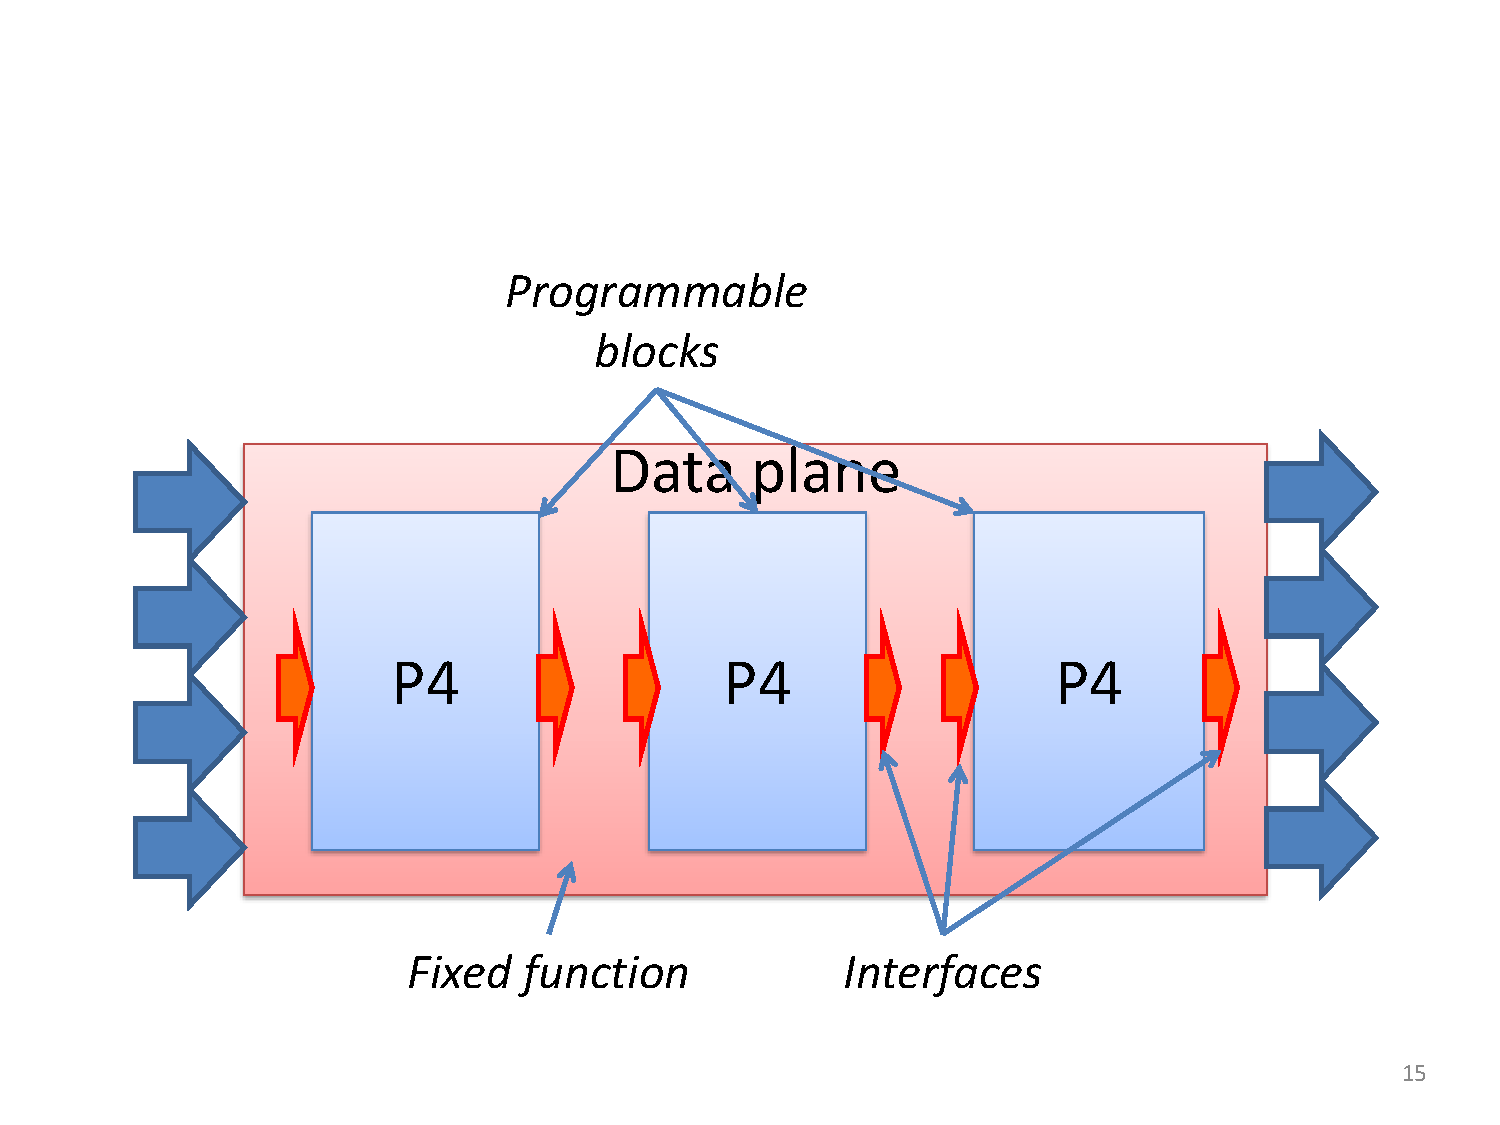
\includegraphics[width=.5\textwidth,clip,trim=1in 0.9in
      .8in 1.8in]{architecture.pdf}}
  \caption{\sl Generic abstract packet-processing engine programmable
    in P4.  The blue blocks labeled with P4 are programmable in P4; the
    surrounding red block is fixed-function
    logic.\label{fig:architecture}}
\end{figure}

Figure~\ref{fig:architecture} is an abstract view of how a P4 program
interacts with the data-plane of a packet-processing engine.  The
data-plane is a fixed-function device that provides several
programmable ``holes''.  The user writes a P4 program to ``fill'' each
hole.  The target manufacturer describes the interfaces between the
programmable blocks and the surrounding fixed-function blocks.  These
interfaces are target-specific.  Note that the fixed-function part can
be software, hardware, firmware, or a mixture.

A P4 architecture file is expected to contain declarations of types,
constants, and a description of the control and parser blocks that the
users need to implement.  Sections~\ref{sec:ebpf} and~\ref{sec:xdp}
contain examples P4 architecture description files.

\subsection{eBPF for network processing}

\mycomment{(This section is adapted from~\cite{p4-ebpf-backend}.) }
eBPF is a
acronym that stands for Extended Berkeley Packet Filters. In essence
eBPF is a low-level programming language (similar to machine code);
eBPF programs are traditionally executed by a virtual machine that
resides in the Linux kernel. eBPF programs can be inserted and removed
from a live kernel using dynamic code instrumentation. The main
feature of eBPF programs is their static safety: prior to execution
all eBPF programs have to be validated as being safe, and unsafe
programs cannot be executed. A safe program provably cannot compromise
the machine it is running on:
\begin{itemize}
\item it can only access a restricted set of memory regions (verified
  either statically or through inline bounds checks using
  software-fault isolation techniques~\cite{wahbe:93}),
\item it can run only for a limited amount of time; during execution
  it cannot block, sleep or take any locks,
\item it cannot use any kernel resources with the exception of a
  limited set of kernel services which have been specifically
  whitelisted, including operations to manipulate tables (described
  below)
\end{itemize}

\subsubsection{Kernel hooks}

eBPF programs are inserted into the kernel using hooks; their
execution is triggered when the flow of control reaches these hooks:

\begin{itemize}
\item function entry points can act as hooks; attaching an eBPF
  program to a function foo() will cause the eBPF program to execute
  every time some kernel thread executes foo().

\item eBPF programs can also be attached using the Linux Traffic
  Control (TC) subsystem, in the network packet processing
  datapath. Such programs can be used as TC classifiers and actions.

\item eBPF programs can also be attached to sockets or network
  interfaces. In this case they can be used for processing packets
  that flow through the socket/interface.
\end{itemize}

\subsubsection{eBPF Maps}

The eBPF runtime exposes a bi-directional kernel-userspace data
communication channel, called maps.  eBPF maps are essentially
key-value tables, where keys and values are arbitrary fixed-size
bitstrings.  The key width, value width and the maximum number of
entries that can be stored in a map are declared at map creation time.

In user-space maps are are exposed as file descriptors. Both user- and
kernel-space programs can manipulate maps by inserting, deleting,
looking up, modifying, and enumerating entries.

In kernel space the keys and values are exposed as pointers to the raw
underlying data stored in the map, whereas in user-space the
pointers point to copies of the data.

\subsubsection{Concurrency}

The execution of an eBPF program is triggered by the corresponding
kernel hook; multiple instances of the same kernel hook can be running
simultaneously on different cores.

A map may be accessed simultaneously by multiple instances of the same
eBPF program running as separate kernel threads on different cores.
eBPF maps are native kernel objects, and access to the map contents is
protected using the kernel RCU mechanism. This makes access to table
entries safe under concurrent execution; for example, the memory
associated to a value cannot be accidentally freed while an eBPF
program holds a pointer to the respective value.  However, accessing
maps is prone to data races; since eBPF programs cannot use locks,
some of these races often cannot be avoided.

\subsection{XDP: eXpress Data Path}\label{sec:xdp-background}

An XDP program is special case of an eBPF program for processing
network packets, which attaches to the lowest levels of the networking
stack.  XDP was designed initially for quickly computing whether a
packet should be dropped, before too many kernel resources have been
allocated, to prevent denial-of-service attacks.  An XDP program can
inspect a network packet right after the DMA engine copies the packet
from the network card.

XDP program can access eBPF maps.  The kernel expects an XDP program
to return the decision taken about the processed packet, one of the
following values:

\begin{description}
\item[XDP\_DROP] the packet should be immediately dropped,
\item[XDP\_TX] bounce the received packet back on the same port it arrived on,
\item[XDP\_PASS] continue to process the packet using,
  the normal kernel network stack,
\item[XDP\_REDIRECT] forward the packet to another port.
\end{description}

\subsection{Comparison of P4 and eBPF}

A very thorough evaluation of eBPF for writing networking programs can
be found in~\cite{minao-hspr18}.  P4 and eBPF share many features.
Table~\ref{table:compare} shows a comparison of the high-level
features of both languages.

\begin{table}[t]
  \footnotesize
  \begin{center}
  \begin{tabular}{|p{1.5cm}|p{2.7cm}|p{2.7cm}|} \hline
    \textbf{Feature} & \textbf{P4} & \textbf{eBPF} \\ \hline \hline
    Targets & ASIC, software, FPGA, NIC & Linux kernel \\ \hline
    Licensing & Apache & GPL \\ \hline
    Tools & Compilers, simulators & LLVM back-end, verifier \\ \hline
    Level & High & Low \\ \hline
    Safe  & Yes & Yes \\ \hline
    Safety & Type system & Verifier \\ \hline
    Resources & Statically allocated & Statically allocated \\ \hline
    Policies & Match-action tables & Key-value eBPF maps \\ \hline
    Extern helpers & Target-specific & Hook-specific \\ \hline
    Execution model & Event-driven & Event-driven \\ \hline
    Control-plane API & Synthesized by compiler & eBPF maps \\ \hline
    Concurrency & No shared R/W state & Maps are thread-safe \\ \hline
  \end{tabular}
  \caption{Feature comparison between P4 and eBPF.}\label{table:compare}
  \end{center}
\end{table}

P4 was designed as a language for programming switching devices,
working mostly at levels L2 and L3 of the networking stack.  While P4
is being used for programming network end-points, e.g., smart NICs,
some end-point functionality cannot be naturally expressed in P4
(e.g., TSO, encryption, deep packet inspection).

\begin{table*}[t]
  \footnotesize
  \begin{center}
  \begin{tabular}{|l|l|l|} \hline
    \textbf{Limitation} & \textbf{P4} & \textbf{eBPF} \\ \hline \hline
    Loops & Parsers & Tail call \\ \hline
    Nested headers & Bounded depth & Bounded depth \\ \hline
    Multicast/broadcast & External & Helpers \\ \hline
    Packet segmentation & No & No \\ \hline
    Packet reassembly &	No & No \\ \hline
    Timers/timeouts/aging & External & No \\ \hline
    Queues & No & No \\ \hline
    Scheduling & No & No \\ \hline
    Data structures & No & No \\ \hline
    Payload processing & No & No \\ \hline
    State & Registers/counters & Maps \\ \hline
    Iterating over packet payload & No & No \\ \hline
    Wildcard matches & Yes & No \\ \hline
    Table/map writes & Control-plane only & Data-plane and control-plane \\ \hline
    Iteration over table/map values & Control-plane only & Control-plane only \\ \hline
    Synchronization (data/data, data/control)  & No & No \\ \hline
    Resources & Statically allocated & Limited stack and buffer \\ \hline
    Control-plane support & Complex, including remote & Simple \\ \hline
    Safety & Safe & Verifier limited to small programs \\ \hline
    Compiler & Target-dependent & LLVM back-end \\ \hline
  \end{tabular}
  \caption{Comparison of the limitations of P4 and
    eBPF.}\label{table:limitations}
  \end{center}
\end{table*}

Many of these P4 limitations are shared with eBPF.  In general, while
P4 and eBPF are good for performing relatively simple packet
filtering/rewriting, neither language is good enough to implement a
full end-point networking stack.  Table~\ref{table:limitations}
compares the limitations of P4 and eBPF.

\section{Compiling P4 to eBPF}\label{sec:compilation}

In this section we describe two open-source compilers that translate
P4 programs in stylized C programs, that can in turn be compiled into
eBPF programs using the LLVM eBPF back-end.

\subsection{Packet filters with eBPF}\label{sec:ebpf}

The eBPF back-end is part of the P4 reference compiler
implementation~\cite{p4-ebpf-backend}.  This back-end targets a
relatively simple packet filter architecture.  The following is the
architectural model of an eBPF packet filter expressed in P4.  This
architecture comprises a parser and a control block; the control block
must produce a Boolean value which indicates whether the packet is
accepted or not.

\begin{lstlisting}
#include <core.p4>

extern CounterArray {
    CounterArray(bit<32> max_index, bool sparse);
    void increment(in bit<32> index);
}

extern array_table {
    array_table(bit<32> size);
}

extern hash_table {
    hash_table(bit<32> size);
}

parser parse<H>(packet_in packet, out H headers);
control filter<H>(in H headers, out bool accept);

package ebpfFilter<H>(parse<H> prs,
                      filter<H> filt);
\end{lstlisting}

The following listing shows a P4 program written for this architecture
that counts the number of IPv4 packets that are encountered.

\begin{lstlisting}
#include <core.p4>
#include <ebpf_model.p4>

typedef bit<48> EthernetAddress;
typedef bit<32> IPv4Address;

header Ethernet {
    EthernetAddress dstAddr;
    EthernetAddress srcAddr;
    bit<16> etherType;
}

// IPv4 header without options
header IPv4 {
    bit<4>       version;
    bit<4>       ihl;
    bit<8>       diffserv;
    bit<16>      totalLen;
    bit<16>      identification;
    bit<3>       flags;
    bit<13>      fragOffset;
    bit<8>       ttl;
    bit<8>       protocol;
    bit<16>      hdrChecksum;
    IPv4Address  srcAddr;
    IPv4Address  dstAddr;
}

struct Headers {
    Ethernet eth;
    IPv4     ipv4;
}

parser prs(packet_in p, out Headers headers) {
    state start {
        p.extract(headers.eth);
        transition select(headers.eth.etherType) {
            0x800 : ip;
            default : reject;
        }
    }

    state ip {
        p.extract(headers.ipv4);
        transition accept;
    }
}

control pipe(in Headers headers, out bool pass) {
    CounterArray(32w10, true) ctr;

    apply {
        if (headers.ipv4.isValid()) {
            ctr.increment(headers.ipv4.dstAddr);
            pass = true;
        } else
            pass = false;
    }
}

ebpfFilter(prs(), pipe()) main;
\end{lstlisting}

Compilation to C is fairly straightforward; the generated C program is
always memory-safe, using bounds-checks for all packet accesses.  For
the entire P4 program a single C function is generated which returns a
Boolean value.  Table~\ref{table:translation} shows how each P4
construct is converted to a C construct.  Currently programs with
parser loops are rejected, but a parser loop unrolling pass (under
development) will allow such programs to be compiled.

\begin{table}[h]
  \footnotesize
  \begin{center}
  \begin{tabular}{|l|p{5cm}|} \hline
    \textbf{P4 construct} & \textbf{C Translation} \\ \hline \hline
    \texttt{header} & \texttt{struct} with an additional \texttt{valid} bit \\ \hline
    \texttt{struct} & \texttt{struct} \\ \hline
    parser state    & block statement \\ \hline
    state transition & \texttt{goto} statement \\ \hline
    \texttt{extract} call & load/shift/mask data from packet \\ \hline
    table & 2 eBPF maps --- one for actions, one for the default action \\ \hline
    table key type & \texttt{struct} type \\ \hline
    \texttt{action} & tagged \texttt{union} with action parameters \\ \hline
    \texttt{action} parameters & \texttt{struct} \\ \hline
    \texttt{action} body & block statement \\ \hline
    table \texttt{apply} & lookup in eBFP map + \texttt{switch} statement with all actions \\ \hline
    counters & eBPF map \\ \hline
  \end{tabular}
  \end{center}
  \caption{Compiling P4 constructs to C.}\label{table:translation}
\end{table}

\subsection{Packet forwarding with XDP}\label{sec:xdp}

A second P4 to C compiler is available as an open-source
project:~\cite{p4-xdp-backend}.  This compiler extends the eBPF
compiler from Section~\ref{sec:ebpf}.  This compiler can target either
a packet filter, or a packet switch.  The following listing shows the
XDP architectural model targeted by this compiler.  You can see that a
P4 XDP program can (1) return to the kernel one of the 4 outcomes
described in Section~\ref{sec:xdp-background}, and (2) it can also
modify the packet itself, by inserting, modifying or deleting headers.

\begin{lstlisting}
#include <ebpf_model.p4>
enum xdp_action {
  XDP_ABORTED,
  XDP_DROP,
  XDP_PASS,
  XDP_TX
}
struct xdp_input { bit<32> input_port }

struct xdp_output {
  xdp_action output_action;
  bit<32> output_port;
}

parser xdp_parse<H>(packet_in packet,
                    out H headers);
control xdp_switch<H>(inout H hdrs,
                      in xdp_input i,
                      out xdp_output o);
control xdp_deparse<H>(in H headers,
                       packet_out packet);

package xdp<H>(xdp_parse<H> p,
               xdp_switch<H> s,
               xdp_deparse<H> d);
\end{lstlisting}

\section{Testing eBPF programs}\label{sec:testing}
The compiler integrates an end-to-end testing framework to verify the 
correctness of a P4-eBPF/XDP program. The framework consists of a user space 
and a kernel testing pipeline. Both run a test from the compilation 
till the actual runtime deployment of a P4 program.

\subsection{Why Test in User-Space?}
Testing in user space isolates the specification of the eBPF program from the
implementation. It is primarily intended to test the correctness of the
compiler and the generated C code without interference of the kernel verifier
and tooling. The user space testing framework does not depend on the LLVM
compiler or specific kernel version. It also does not require usage of iproute2 
tooling such as tc or ip. Our aim is to ensure that a P4 program is functionally
equivalent to its corresponding XDP C-code.

Testing in user space also ensures debugging simplicity for the average
user. Tools such as GDB, valgrind, wireshark, or simple output statements
are readily available.

\subsection{The Simple Test Framework}
\begin{figure}
	\centering
	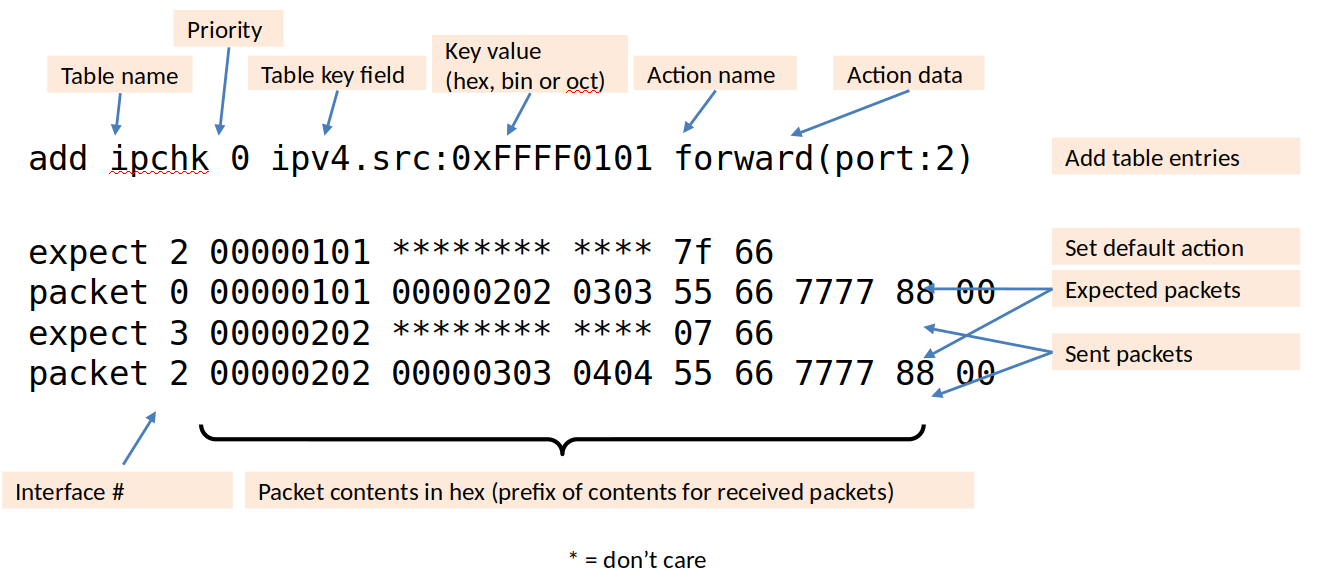
\includegraphics[width=\linewidth]{stf}
	\caption{Simple testing framework program fragment for exercising P4 programs.}
	\label{fig:stf}
\end{figure}
The simple test framework (STF) is a dataplane verification language. 
An STF template defines a set of actions which are sequentially executed on the 
dataplane.

An example STF action is \texttt{packet}. \texttt{packet} describes the 
byte content of an inbound Ethernet frame and the port which will receive the 
packet.
Its counterpart, \texttt{expect}, defines which port will send out an Ethernet 
frame. This implies we \textit{expect} our dataplane to forward the frame 
given by \texttt{packet} to the port in the command.
The action \texttt{add} on the other hand is a simple PUT operation on 
dataplane tables. It describes which table to update and what key-value pair to 
insert.

While its original purpose is to assess switching and forwarding behavior, STF 
templates can also be used to test eBPF programs in isolation. The P4 compiler 
features a parser, which pre-processes the templates and generates an ordered 
command list. This list is interpreted by the eBPF testing framework, 
which produces pcap files from the \texttt{packet} commands and converts 
\texttt{add} operations into eBPF map syscalls.
Table \ref{table:stf} describes the full list of commands that are currently 
supported.

\paragraph{Example}
An example of an STF template can be seen in Figure \ref{fig:stf}. \texttt{add} 
defines that, if the IPv4 source address of a packet matches with the key in 
table \texttt{ipchk}, we forward the packet to 
port 2. After the table update, the template specifies to insert packets on 
port 0 and 2 and to expect output packets on port 2 and 3.


\begin{table*}[h]
	\begin{center}
		\begin{tabular}{|l|p{9cm}|} \hline
			\textbf{Command} & \textbf{Description} \\ \hline \hline
			\textbf{packet} port data & Insert a frame of bytes
			\textit{data} into port \textit{port}.    \\ \hline
			\textbf{expect} port data & Expect a frame of bytes
			\textit{data} on port \textit{port}.  \\ \hline
			\textbf{add} tbl priority match action & Insert a
			match-action entry with key \textit{match} and action
			\textit{action} into table \textit{tbl}. \\ \hline
			\textbf{setdefault} tbl action & Set the default action for table
			\textit{tbl}. \\
			\hline
			\textbf{check\_counter} tbl\_name key == n & Check if the value on
			the entry \textit{key} in counter table \textit{tbl} matches
			\textit{n}.  \\
			\hline
			\textbf{wait} & Pause any operation for a second. \\ \hline
		\end{tabular}
		\caption{The STF command palette.}\label{table:stf}
	\end{center}
\end{table*}

\subsection{The Test Runtime}
A P4C-XDP test is an end-to-end verification of all stages of 
the compilation pipeline. This includes verifying that the P4 code does 
compile, that the generated eBPF/XDP C is correct, and that the actual runtime 
behavior of the loaded program matches expectations.

\subsubsection{Architecture}
The test infrastructure is designed to be flexible and independent of the 
target backend. New testing frameworks can be added by creating a target file 
and linking it to the P4C test target folder. Each test will pass through five 
abstract test stages:\\

\noindent\textbf{compile-p4}\\ Compile the P4 file to a dataplane binary. \\
\textbf{parse-stf}\\ Parse the stf file and interpret the output. \\
\textbf{compile-dataplane}\\ Load the P4 binary and create a runtime.\\
\textbf{run}\\ Start the runtime and read in the STF file inputs.\\
\textbf{check-results}\\ Compare the results with the STF 
expectations.\\

The implementation of these stages is up to the compiler backend.
Currently, both eBPF/XDP kernel and user space targets are supported.

The user space testing framework defines a set of eBPF wrappers to approximate 
the kernel implementation. eBPF maps are implemented as simple hash maps, the 
map file descriptor API is emulated by a common registry. Functionality is 
limited and only extends to the minimal eBPF map operations necessary for 
filtering and classifying.

Every target in the eBPF compiler is required to implement a custom 
\textit{target header}. This target header specifies how macros in the eBPF 
source file are expanded. For example, \texttt{ebpf\_test.h} defines 
\texttt{BPF\_MAP\_LOOKUP\_ELEM} to call into the userspace registry whereas 
\texttt{ebpf\_kernel.h} defines the function as the standard eBPF system call.

\subsubsection{Running a Test}
A test requires only an STF template and a P4 program as input. The 
remaining files are generated or linked. The five testing stages are 
implemented as follows:\\

\noindent\textbf{compile-p4}\\
Depending on the backend the P4 program is either compiled to eBPF or 
to XDP C-Code. A header file accompanies the generated program. This stage 
verifies that the P4 program matches the expected syntax.\\ 
\textbf{parse-stf}\\
The framework parses the associated STF file and generates a set of input pcap 
files per port. The expected output packets are stored in a map for later use. 
In addition, all \texttt{add} operations are converted to eBPF map calls and 
exported as control file.\\
\textbf{compile-dataplane}\\
Once the P4 and STF file have been parsed, the framework compiles 
the eBPF C program, the eBPF wrappers, and the control plane operations into a 
test runtime.

This runtime initializes all eBPF tables with entries specified by the STF 
file, then "runs" the dataplane by processing a set of input packets.
As input the runtime takes a set of pcap files, which are spliced into per-port 
lists and individually inserted into the datapath.
As the pcapng format, which contains port information as packet metadata, is 
not yet supported by libpcap, we identify the input port of a pcap file by
its filename.

In addition to creating the runtime, the kernel version compiles the eBPF/XDP 
program to an eBPF object using clang and llvm.\\
\textbf{run}\\
At this point, the user and kernel frameworks diverge in behavior.

In the user space version, packets are converted to a mock-sk\_buff structure 
and then directly passed into the to-be-tested eBPF/XDP function call. The 
output result is recorded and written to per-port output pcap files.

The kernel framework, however, is intended to verify the correctness of an 
eBPF/XDP object in relation to the host kernel. This results in a more complex 
pipeline (See Figure \ref{fig:kernel_test}). 
Before the eBPF program is loaded, the framework creates a bridge running in an 
network namespace. Isolation via a namespace ensures that existing 
virtual interfaces and eBPF maps do not conflict with the test in question.
\texttt{n} virtual interfaces are attached to the bridge, corresponding to 
the highest port identifier defined in the STF file.

The compiled eBPF object is then loaded into all ports using \texttt{tc} or 
\texttt{ip}. Instead of directly calling into the eBPF program, the kernel 
runtime writes the packet to the associated port using raw sockets. The output 
results are recorded by sniffing on the interfaces via tcpdump.\\
\textbf{check-results}\\
After the program has completed, the results are collected and compared with 
the expected packets defined by the STF template. If the output port or the 
dataframe content does not match the specification, the test returns an error 
code and is marked as failed.

Both the user and kernel space runtime do not support testing for counters 
and table state yet. We have planned these extensions as future work.
\begin{figure}
	\centering
	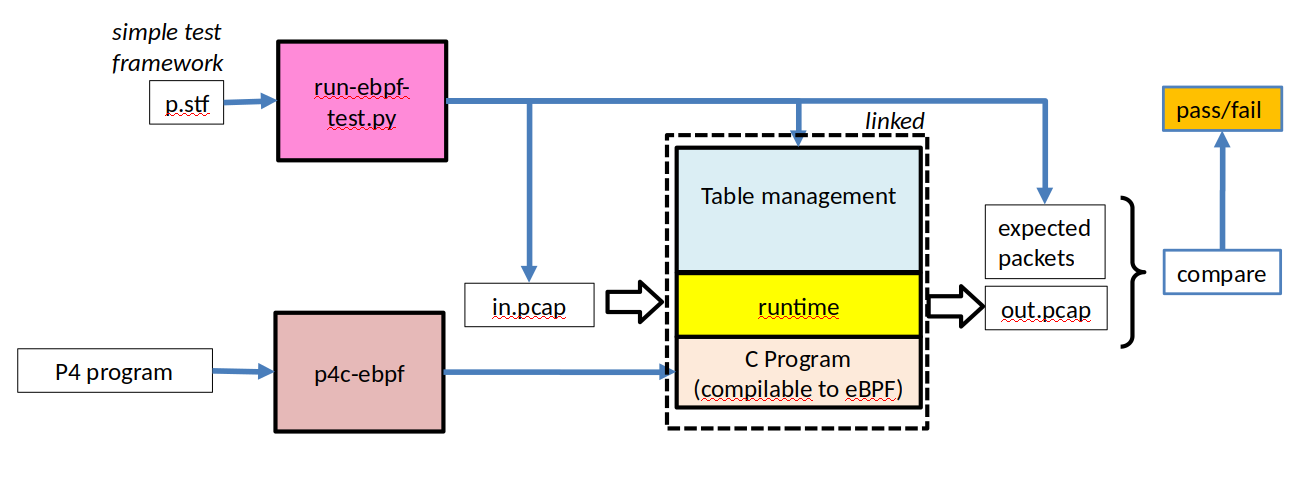
\includegraphics[width=\linewidth]{user_test}
	\caption{User-level testing of the C programs generated by the P4 compilers.}
	\label{fig:user_test}
\end{figure}
\begin{figure}
	\centering
	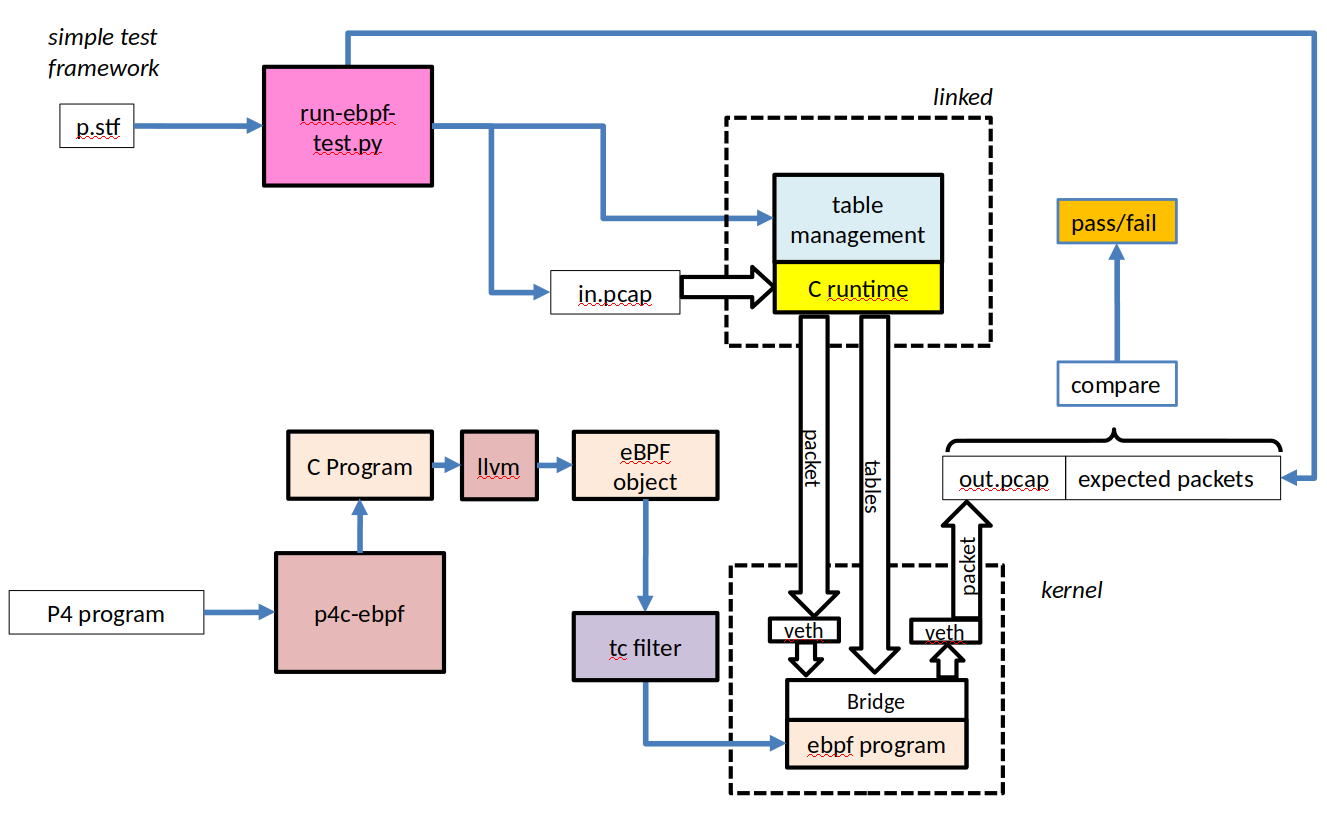
\includegraphics[width=\linewidth]{kernel_test}
	\caption{Kernel-level testing of the C programs generated by the P4 
	compilers.}
	\label{fig:kernel_test}
\end{figure}
\subsubsection{Using the Test Runtime}
The test framework can be used independently to verify eBPF and XDP programs. 
[TODO] Talk about how you test raw ebpf C programs with having a P4 template. 
The idea is that we can use the backend to also just test random eBPF/XDP 
programs with our compiler. I have not been able to implement this yet.
Also talk how to use:
\begin{lstlisting}[language=bash]
make -f p4c/backends/ebpf/runtime/kernel.mk \
	BPFOBJ=out.o P4FILE=PROGRAM.p4
\end{lstlisting}
to directly compile P4 to an eBPF object.

\section{Experimental results}\label{sec:results}
\subsection{Testbed}
All of our performance results use a hardware test bed that consists of
two Intel Xeon E5 2440 v2 1.9GHz servers, each with 1 CPU socket and
8 physical cores with hyperthreading enabled.
Each target server has an Intel 10GbE X540-AT2 dual
port NIC, with the two ports of the Intel NIC on one server connected
to the two ports on the identical NIC on the other server.
We installed p4c-xdp on one server, the {\em target server}, and
attached the XDP program to the port that receives the packets
The other server, the {\em source server}, generates packets
at the maximum 10~Gbps packet rate of 14.88~Mpps using the DPDK-based
TRex~\cite{trex} traffic generator.  The source server sends minimum
length 64-byte packets in a {\em single} UDP flow to one port of the
target server, and receives the forwarded packets on the same port.
At the target server, we use only one core to process all packets.
Every packet received goes through the pipeline specified in P4.

We use the sample p4 programs in the tests directory and the following
metrics to understand the performance impact of the P4-generated XDP
program:
\begin{itemize}
\item Packet Processing Rate (Mpps): Once the XDP program finishes
  processing the packet, it returns one of the actions mentioned in
  section~\ref{sec:background}.  When we want to count the number of
  packets that can be dropped per second, we modify each p4 program to
  always return XDP\_DROP.
\item CPU Utilization: Every packet processed by the XDP program is run
  under the per-core software IRQ daemon, named
  \texttt{ksoftirqd/\textit{core}}.  All packets are processed by only
  one core with one kthread, the ksoftirqd, and we measure the CPU
  utilization of the ksoftirqd on the core.
\item Number of BPF instructions verified: For each program, we list
  the complexity as the number of BPF instructions the eBPF
  verifier scans.
\end{itemize}

The target server is running Linux kernel 4.19-rc5 and for all our
tests, the BPF JIT (Just-In-Time) compiler is enabled and JIT hardening
is disabled. All programs are compiled with clang 3.8 with llvm 5.0.
For each test program, we use the following
command from iproute2 to load it into kernel:
\begin{lstlisting}[frame=none]
ip link set dev eth0 xdp obj xdp1.o verb
\end{lstlisting}

The Intel 10GbE X540 NIC is running the \texttt{ixgbe} driver with 16 RX queues
set-up. Since the source server is sending single UDP flow, packets
always arrive at a single ring ID.  As a result, we collect the number
of packets being dropped at this ring.

\subsection{Results}

To compute the baseline performance we wrote two small XDP programs by
hand: \texttt{SimpleDrop}, drops all packets by returning
\texttt{XDP\_DROP} immediately.  \texttt{SimpleTX} forwards the packet
to the receiving port returning \texttt{XDP\_TX}.  Each of these
programs consists of only two BPF instructions.

\begin{lstlisting}[frame=none]
    /* SimpleDrop */
    0: (b7) r0 = 1 // XDP_DROP
    1: (95) exit

    /* SimpleTX */
    0: (b7) r0 = 3 // XDP_TX
    1: (95) exit
\end{lstlisting}

After, we attached the following P4 programs to the receiving device:
\begin{itemize}
\item xdp1.p4: Parse Ethernet/IPv4 header, deparse it, and drop.
\item xdp3.p4: Parse Ethernet/IPv4 header, lookup a MAC address
in a map, deparse it, and drop.
\item xdp6.p4: Parse Ethernet/IPv4 header, lookup and get a new TTL value
from eBPF map, set to IPv4 header, deparse it, and drop.
\item xdp7.p4: Parse Ethernet/IPv4/UDP header, write a pre-defined source port
and source IP, recalculate checksum, deparse, and drop.
\item xdp11.p4: Parse Ethernet/IPv4 header, swap src/dst MAC address,
deparse it, and send back to the same port (XDP\_TX).
\item xdp15.p4: Parse Ethernet header, insert a customized 8-byte header,
deparse it, and send back to the same port (XDP\_TX).
\end{itemize}

\begin{table}
\centering
\small
\begin{tabular}{llll}
  \underline{P4 program} & \underline{CPU Util.} & \underline{Mpps} & \underline{Insns./Stack}\\
  SimpleDrop & 75\% & 14.4 & 2/0 \\
  SimpleTX & 100\% & 7.2 & 2/0 \\
  xdp1.p4 &  100\% &  8.1 & 277/256 \\
  xdp3.p4 &  100\% &  7.1 & 326/256 \\
  xdp6.p4 &  100\% &  2.5 & 335/272 \\
  xdp7.p4 &  100\% &  5.7 & 5821/336 \\
  xdp11.p4 &  100\% &  4.7  & 335/216 \\
  xdp15.p4 &  100\% &  5.5 & 96/56\\
\end{tabular}
\caption{\footnotesize Performance of XDP program generated by
  p4c-xdp compiler using single core.}
\label{tab:perf}
\end{table}

As shown in Table~\ref{tab:perf}, xdp1.p4 allows us to measure the
overhead introduced by parsing and deparsing: a drop from 14.4~Mpps to
8.1~Mpps.  xdp3.p4 reduces the rate by another million PPS due to the
eBPF map lookup (this operation always return NULL, no value from the
map is accessed).  xdp6.p4 has significant overhead because it
accesses a map, finds a new TTL value, and writes to the IPv4 header.
Interestingly, although xdp7.p4 does extra parsing to the UDP header
and checksum recalculation, it has only a moderate overhead because of
the lack of map accesses.

Finally, xdp11.p4 and xdp15.p4 show the transmit (XDP\_TX)
performance.  Compared with xdp11, xdp15.p4 invokes the
bpf\_adjust\_head helper function to reset the pointer for extra
bytes.  It does not incur much overhead because there
is already a reserved space in front of every XDP packet frame.

\subsection{Performance Analysis}

To further understand the performance overhead of programs generated
by p4c-xdp, we started broke down the CPU utilization. We used the Linux
perf tool on the process ID of the ksoftirqd that shows 100\%:
\begin{lstlisting}[frame=none]
perf record -p <pid of ksoftirqd> sleep 10
\end{lstlisting}


\noindent The following output shows the profile of xdp1.p4:
{\scriptsize
\begin{verbatim}
 83.19% [kernel.kallsyms] [k] ___bpf_prog_run
 8.14%  [ixgbe]           [k] ixgbe_clean_rx_irq
 4.82%  [kernel.kallsyms] [k] nmi
 1.48%  [kernel.kallsyms] [k] bpf_xdp_adjust_head
 1.07%  [kernel.kallsyms] [k] __rcu_read_unlock
 0.40%  [ixgbe]           [k] ixgbe_alloc_rx_buffers
\end{verbatim}
}

This confirms that most of the CPU cycles are spent on executing the
XDP program, \texttt{\_\_\_bpf\_prog\_run}, which caused us to investigate the 
eBPF C code of xdp1.p4.

\begin{table}
\centering
\small
\begin{tabular}{llll}
  \underline{P4 program} & \underline{CPU Util.} & \underline{Mpps} & \underline{Insns./Stack}\\
  xdp1.p4 &  77\% &  14.8 & 26/0 \\
  xdp3.p4 &  100\% &  13 & 100/16 \\
  xdp6.p4 &  100\% &  12 & 98/40 \\
\end{tabular}
\caption{\footnotesize Performance of XDP program without deparser.}
\label{tab:perf2}
\end{table}

After commenting out the deparser C code, performance increases
significantly (see Table~\ref{tab:perf2}).  In the generated
code, the p4c-xdp compiler always writes back the entire packet
content, even when the P4 program does not modify any fields.  In
addition, the parser/deparser incur byte-order translation, e.g.,
htonl, ntohl.  This could be avoided by always using network
byte-order in P4 and XDP.  We plan to implement optimizations to
reduce this overhead.

\section{Lessons learned}\label{sec:conclusions}

In general, our development experience is mirrored by the lessons described
in~\cite{minao-hspr18} and ~\cite{bertin-netdev17}.

\paragraph{No multi-/broadcast support}
While XDP is able to redirect single frames it does not have the ability to
clone and redirect packets similar to \texttt{bpf\_clone\_redirect}. This makes
development of more sophisticated P4 forwarding programs problematic.

\paragraph{The stack size is too small}
More complex XDP programs are rejected by the verifier despite being
safe.  This is a particular challenge when attempting to implement
network function chaining or more advanced pipelined packet processing
in a single XDP program.  The LLVM eBPF code generator allocates 8
stack bytes even for 1 byte variables, increasing the stack usage
significantly.

\paragraph{Generic XDP and TCP}
Our testing framework uses virtual Linux interfaces and generic XDP~\cite{genericxdp}
to verify XDP programs.
Unfortunately, we are unable to test TCP streams as the protocol is not
supported by this driver~\cite{xdptcp}.
Any program loaded by generic XDP operates after the creation of
the \texttt{skb} and requires the original packet data. Since TCP clones every
packet and passes the unmodifiable \texttt{skb} clone,  generic XDP is
bypassed and never receives the datagram.

\paragraph{Using libbpf userspace library}
Creating of compilation of eBPF programs in userspace requires substantial
effort. Many function calls and variables available in sample programs are not
available as C library and currently the p4c-xdp project copied these utilities
from kernel code or assembled from various online sources. We plan to switch to
use libbpf to control and manage the eBPF programs and maps.

\paragraph{Persistent eBPF maps in namespaces}
When using eBPF programs in namespaces, maps exported via tc do not
persist across \texttt{ip netns exec} calls. The consequence is that
any program has to be run in a single shell command, otherwise the
eBPF map becomes unusable despite the continued existence of the
namespace.


\end{document}
